\documentclass[12pt]{article}
\usepackage{fullpage}
\usepackage{titlesec}
\usepackage{tikz}
\usepackage{amsfonts,amssymb}
\usepackage{amsmath}
\usepackage{comment}
\usetikzlibrary{automata, positioning}

\input ../libraries/mac.tex
\input ../libraries/mathmac.tex

\begin{document}
\pagestyle{plain}
\titleformat{\subsection}[runin]
  {\normalfont\large\bfseries}{\thesubsection}{1em}{}
\titleformat{\subsubsection}[runin]
  {\bfseries}{}{1em}{}

\title{Homework 6}
\author{Brooke Fugate, Michael O'Connor, Rohan Shah}
\date{}

\maketitle

\section*{Problem B2}
\subsection*{(i)}
NFA $N_{C_G}$ for the grammer $G$:
\newline
\begin{center}
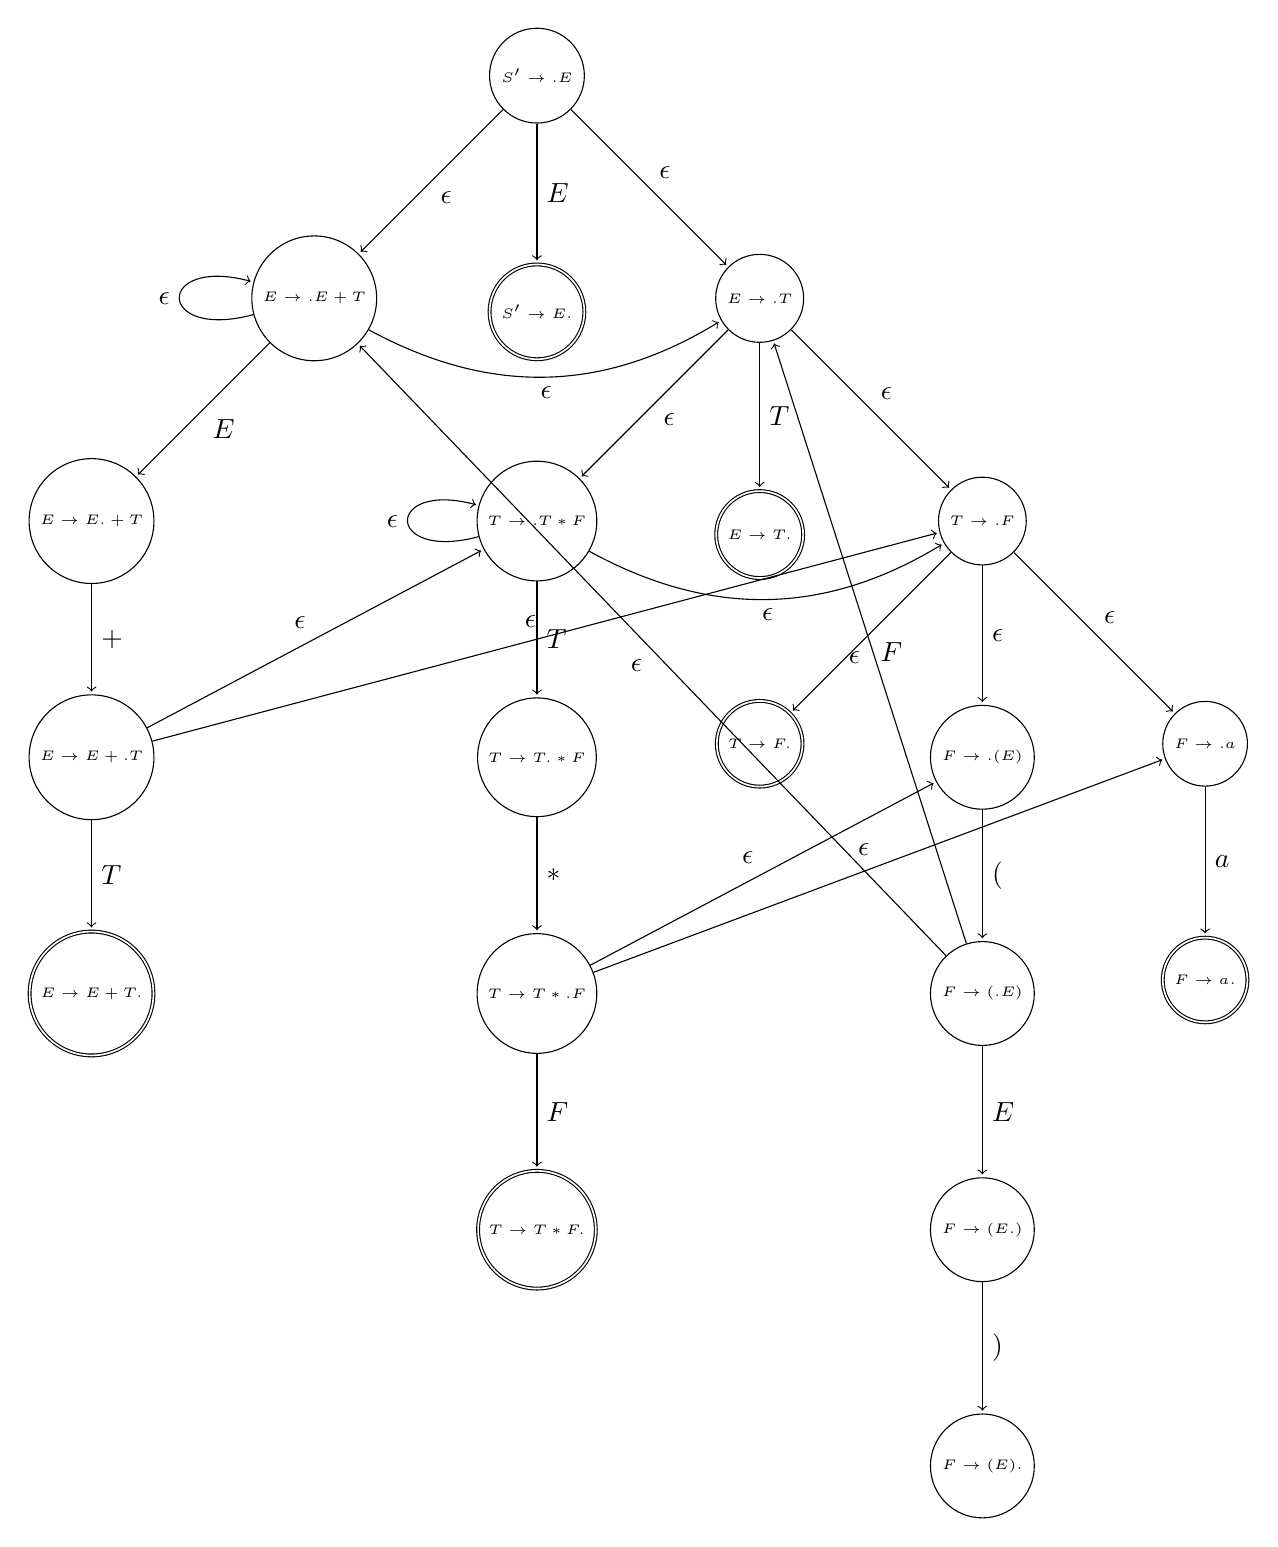
\begin{tikzpicture}[shorten >=1pt, node distance=3cm, on grid, auto]
  \node[state] (q0) {\tiny $S' \rightarrow .E$};
  \node[state, accepting] (q1) [below=of q0] {\tiny $S' \rightarrow E.$};
  \begin{scope}[node distance=4cm]
  \node[state] (q2) [below left=of q0] {\tiny $E \rightarrow .E+T$};
  \node[state] (q3) [below right=of q0] {\tiny $E \rightarrow .T$};
  \node[state] (q4) [below left=of q2] {\tiny $E \rightarrow E.+T$};
  \end{scope}
  \node[state, accepting] (q5) [below=of q3] {\tiny $E \rightarrow T.$};
  \begin{scope}[node distance=4cm]
  \node[state] (q6) [below left=of q3] {\tiny $T \rightarrow .T*F$};
  \node[state] (q7) [below right=of q3] {\tiny $T \rightarrow .F$};
  \end{scope}
  \node[state] (q8) [below=of q4] {\tiny $E \rightarrow E+.T$};
  \node[state] (q9) [below=of q6] {\tiny $T \rightarrow T.*F$};
  \node[state] (q11) [below=of q7] {\tiny $F \rightarrow .(E)$};
  \begin{scope}[node distance=4cm]
  \node[state, accepting] (q10) [below left=of q7] {\tiny $T \rightarrow F.$};
  \node[state] (q12) [below right=of q7] {\tiny $F \rightarrow .a$};
  \end{scope}
  \node[state, accepting] (q13) [below=of q8] {\tiny $E \rightarrow E+T.$};
  \node[state] (q14) [below=of q9] {\tiny $T \rightarrow T*.F$};
  \node[state] (q15) [below=of q11] {\tiny $F \rightarrow (.E)$};
  \node[state, accepting] (q16) [below=of q12] {\tiny $F \rightarrow a.$};
  \node[state, accepting] (q17) [below=of q14] {\tiny $T \rightarrow T*F.$};
  \node[state] (q18) [below=of q15] {\tiny $F \rightarrow (E.)$};
  \node[state] (q19) [below=of q18] {\tiny $F \rightarrow (E).$};

  \path[->]
  (q0) edge node {$E$} (q1)
  (q0) edge node {$\epsilon$} (q2)
  (q0) edge node {$\epsilon$} (q3)
  (q2) edge node {$E$} (q4)
  (q2) edge [loop left] node {$\epsilon$} (q2)
  (q2) edge [bend right] node [below] {$\epsilon$} (q3)
  (q3) edge node {$T$} (q5)
  (q3) edge node {$\epsilon$} (q6)
  (q3) edge node {$\epsilon$} (q7)
  (q4) edge node {$+$} (q8)
  (q6) edge node {$T$} (q9)
  (q6) edge [loop left] node {$\epsilon$} (q6)
  (q6) edge [bend right] node [below] {$\epsilon$} (q7)
  (q7) edge node {$F$} (q10)
  (q7) edge node {$\epsilon$} (q11)
  (q7) edge node {$\epsilon$} (q12)
  (q8) edge node {$T$} (q13)
  (q8) edge node {$\epsilon$} (q6)
  (q8) edge node {$\epsilon$} (q7)
  (q9) edge node {$*$} (q14)
  (q11) edge node {$($} (q15)
  (q12) edge node {$a$} (q16)
  (q14) edge node {$F$} (q17)
  (q14) edge node {$\epsilon$} (q11)
  (q14) edge node {$\epsilon$} (q12)
  (q15) edge node {$E$} (q18)
  (q15) edge node {$\epsilon$} (q2)
  (q15) edge node {$\epsilon$} (q3)
  (q18) edge node {$)$} (q19)
  ;

\begin{comment}
  \node[state] (q2) [right=of q0] {i};
  \node[state] (q1) [above=of q2] {1};
  \node[state] (q3) [below=of q2] {n};
  \node[state, accepting] (q4) [right=of q1] {n+1};
  \node[state, accepting] (q5) [right=of q2] {n+i};
  \node[state, accepting] (q6) [right=of q3] {2n};
  \path[->]
  (q0) edge node {$\epsilon$} (q1)
       edge node {$\epsilon$} (q2)
       edge node {$\epsilon$} (q3)
  (q1) edge [loop left] node {not $a_1$} (q1)
  (q1) edge [bend left] node {$a_1$} (q4)
  (q4) edge [loop right] node {not $a_1$} (q4)
  (q4) edge [bend left] node {$a_1$} (q1)
  (q2) edge [loop above] node {not $a_i$} (q2)
  (q2) edge [bend left] node {$a_i$} (q5)
  (q5) edge [loop right] node {not $a_i$} (q5)
  (q5) edge [bend left] node {$a_i$} (q2)
  (q3) edge [loop left] node {not $a_n$} (q3)
  (q3) edge [bend left] node {$a_n$} (q6)
  (q6) edge [loop right] node {not $a_n$} (q6)
  (q6) edge [bend left] node {$a_n$} (q3)
  ;
\end{comment}
\end{tikzpicture}
\end{center}

\subsection*{(ii)}

\subsection*{(iii)}
\end{document}
